% Graphics for slide 17, in the order the PDF draws them.
\begin{tikzpicture}[remember picture, overlay, x=1bp, y=-1bp,
  shift={(current page.north west)}]
\path[fill=cFFFFFF] (0,0) rectangle (960,540);
\node[anchor=north west, inner sep=0pt] at (56.69,477.21) {
\includegraphics[width=73.42bp, height=37.42bp]{figures/fundamentals-of-hpc/p03-1.png}};
\path[fill=cEE7628,even odd rule] (57.18,55.73) ..controls(57.96,55.73)and(58.6,56.37)..(58.6,57.15) --(58.6,85.5) ..controls(58.6,86.28)and(57.96,86.91)..(57.18,86.91) ..controls(56.4,86.91)and(55.76,86.28)..(55.76,85.5) --(55.76,57.15) ..controls(55.76,56.37)and(56.4,55.73)..(57.18,55.73);
\node[anchor=north west, inner sep=0pt] at (56.69,168.68) {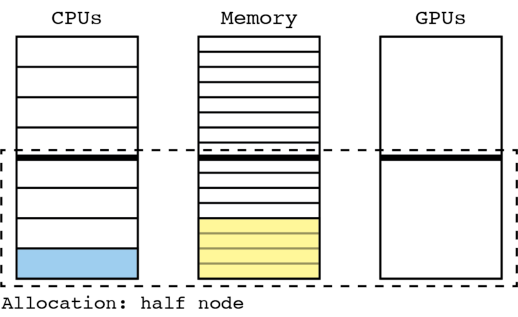
\includegraphics[width=172.43bp, height=105.45bp]{figures/fundamentals-of-hpc/p17-2.png}};
\node[anchor=north west, inner sep=0pt] at (280.29,168.68) {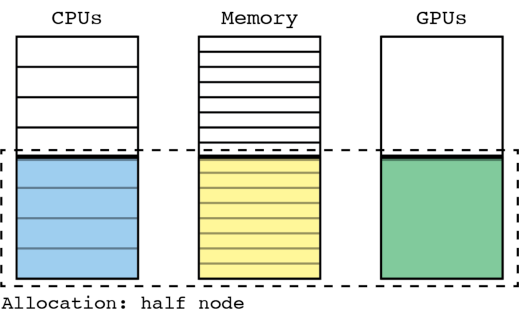
\includegraphics[width=172.43bp, height=105.45bp]{figures/fundamentals-of-hpc/p17-3.png}};
\node[anchor=north west, inner sep=0pt] at (504.46,168.68) {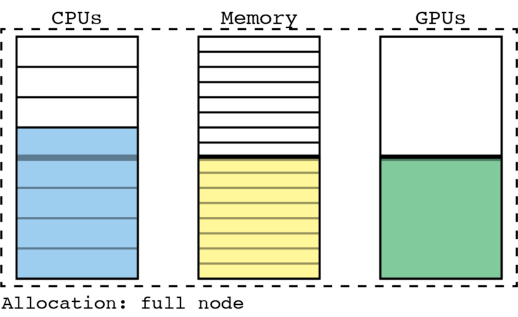
\includegraphics[width=172.43bp, height=105.45bp]{figures/fundamentals-of-hpc/p17-4.png}};
\node[anchor=north west, inner sep=0pt] at (728.84,168.68) {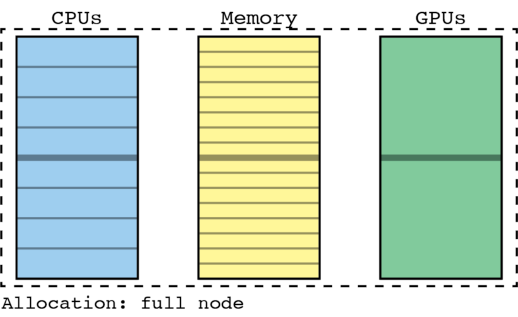
\includegraphics[width=172.43bp, height=105.45bp]{figures/fundamentals-of-hpc/p17-5.png}};
\path[fill=c2CA055,even odd rule] (55.76,100.24) rectangle (130.16,136.24);
\path[fill=c2CA055,even odd rule] (130.16,100.24) rectangle (188.94,136.24);
\path[fill=c2CA055,even odd rule] (188.94,100.24) rectangle (300.77,136.24);
\path[fill=c2CA055,even odd rule] (300.77,100.24) rectangle (356.66,136.24);
\path[fill=c2CA055,even odd rule] (356.66,100.24) rectangle (495.43,136.24);
\path[fill=c2CA055,even odd rule] (495.43,100.24) rectangle (549.29,136.24);
\path[fill=c2CA055,even odd rule] (549.29,100.24) rectangle (705.56,136.24);
\path[fill=c2CA055,even odd rule] (705.56,100.24) rectangle (781.42,136.24);
\path[fill=c2CA055,even odd rule] (781.42,100.24) rectangle (901.27,136.24);
\path[fill=cCDDFD1,even odd rule] (55.76,136.24) rectangle (130.16,163.21);
\path[fill=cCDDFD1,even odd rule] (130.16,136.24) rectangle (188.94,163.21);
\path[fill=cCDDFD1,even odd rule] (188.94,136.24) rectangle (300.77,163.21);
\path[fill=cCDDFD1,even odd rule] (300.77,136.24) rectangle (356.66,163.21);
\path[fill=cCDDFD1,even odd rule] (356.66,136.24) rectangle (495.43,163.21);
\path[fill=cCDDFD1,even odd rule] (495.43,136.24) rectangle (549.29,163.21);
\path[fill=cCDDFD1,even odd rule] (549.29,136.24) rectangle (705.56,163.21);
\path[fill=cCDDFD1,even odd rule] (705.56,136.24) rectangle (781.42,163.21);
\path[fill=cCDDFD1,even odd rule] (781.42,136.24) rectangle (901.27,163.21);
\path[draw=cFFFFFF,line width=1bp,line join=round] (130.16,99.75) --(130.16,163.71);
\path[draw=cFFFFFF,line width=1bp,line join=round] (188.94,99.75) --(188.94,163.71);
\path[draw=cFFFFFF,line width=1bp,line join=round] (300.77,99.75) --(300.77,163.71);
\path[draw=cFFFFFF,line width=1bp,line join=round] (356.66,99.75) --(356.66,163.71);
\path[draw=cFFFFFF,line width=1bp,line join=round] (495.43,99.75) --(495.43,163.71);
\path[draw=cFFFFFF,line width=1bp,line join=round] (549.29,99.75) --(549.29,163.71);
\path[draw=cFFFFFF,line width=1bp,line join=round] (705.56,99.75) --(705.56,163.71);
\path[draw=cFFFFFF,line width=1bp,line join=round] (781.42,99.75) --(781.42,163.71);
\path[draw=cFFFFFF,line width=3bp,line join=round] (55.26,136.25) --(901.77,136.25);
\path[draw=cFFFFFF,line width=1bp,line join=round] (55.76,99.75) --(55.76,163.71);
\path[draw=cFFFFFF,line width=1bp,line join=round] (901.27,99.75) --(901.27,163.71);
\path[draw=cFFFFFF,line width=1bp,line join=round] (55.26,100.25) --(901.77,100.25);
\path[draw=cFFFFFF,line width=1bp,line join=round] (55.26,163.21) --(901.77,163.21);
\path[fill=cFFFFFF,draw=cEE7628,line width=2.25bp,even odd rule] (336.93,280.66) --(396.99,280.66) ..controls(400.68,280.66)and(403.67,282.81)..(403.67,285.45) --(403.67,298.88) ..controls(403.67,301.52)and(400.68,303.67)..(396.99,303.67) --(336.93,303.67) ..controls(333.24,303.67)and(330.25,301.52)..(330.25,298.88) --(330.25,285.45) ..controls(330.25,282.81)and(333.24,280.66)..(336.93,280.66);
\path[fill=cFFFFFF,draw=cEE7628,line width=2.25bp,even odd rule] (112.88,280.73) --(172.94,280.73) ..controls(176.63,280.73)and(179.62,282.88)..(179.62,285.52) --(179.62,298.95) ..controls(179.62,301.59)and(176.63,303.74)..(172.94,303.74) --(112.88,303.74) ..controls(109.19,303.74)and(106.2,301.59)..(106.2,298.95) --(106.2,285.52) ..controls(106.2,282.88)and(109.19,280.73)..(112.88,280.73);
\path[fill=cFFFFFF,draw=cEE7628,line width=2.25bp,even odd rule] (560.64,280.66) --(620.7,280.66) ..controls(624.39,280.66)and(627.38,282.81)..(627.38,285.45) --(627.38,298.88) ..controls(627.38,301.52)and(624.39,303.67)..(620.7,303.67) --(560.64,303.67) ..controls(556.95,303.67)and(553.96,301.52)..(553.96,298.88) --(553.96,285.45) ..controls(553.96,282.81)and(556.95,280.66)..(560.64,280.66);
\path[fill=cFFFFFF,draw=cEE7628,line width=2.25bp,even odd rule] (785.21,280.66) --(845.27,280.66) ..controls(848.96,280.66)and(851.95,282.81)..(851.95,285.45) --(851.95,298.88) ..controls(851.95,301.52)and(848.96,303.67)..(845.27,303.67) --(785.21,303.67) ..controls(781.52,303.67)and(778.53,301.52)..(778.53,298.88) --(778.53,285.45) ..controls(778.53,282.81)and(781.52,280.66)..(785.21,280.66);
\end{tikzpicture}
